\documentclass[12pt, a4]{article}
\usepackage[margin=2cm]{geometry}
\usepackage{parskip}
\usepackage{nameref}
\usepackage{enumitem}
\usepackage{tabularx}
\usepackage{hyperref}
\usepackage[tiny]{titlesec}

\usepackage{amsmath}
\usepackage{amssymb}

\usepackage{fancyhdr}
\usepackage{titling}

\usepackage{pgfplots}
\pgfplotsset{compat=1.16}
\usetikzlibrary{decorations.pathreplacing,positioning}


\usepackage{xcolor}
\usepackage{graphicx}
\usepackage{fancyvrb}
\usepackage{listings}
\usepackage{bm}
\usepackage{xcolor}
\usepackage{optidef}


\xdefinecolor{gray}{rgb}{0.4,0.4,0.4}
\xdefinecolor{blue}{RGB}{58,95,205}
\xdefinecolor{darkgreen}{RGB}{0,100,0}

\newcommand{\lightgray}{black!30}

\newcommand{\plotDomain}{-1:8}

\newcommand{\addPlotLDownCoords}[1]{
	\addplot[mark=none, domain=\plotDomain, color=\lightgray,
	decoration={border,segment length=1mm,amplitude=1.5mm,angle=-135},
	postaction={decorate}
	] coordinates {#1};
	\addplot[mark=none, domain=\plotDomain] coordinates {#1};
}

\newcommand{\addPlotLDown}[1]{
	\addplot[mark=none, domain=\plotDomain, color=\lightgray,
	decoration={border,segment length=1mm,amplitude=1.5mm,angle=-135},
	postaction={decorate}
	] {#1};
	\addplot[mark=none, domain=\plotDomain] {#1};
}

\newcommand{\addPlotRUpCoords}[1]{
	\addplot[mark=none, domain=\plotDomain, color=\lightgray,
	decoration={border,segment length=1mm,amplitude=1.5mm,angle=135},
	postaction={decorate}
	] coordinates {#1};
	\addplot[mark=none, domain=\plotDomain] coordinates {#1};
}

\newcommand{\addPlotRUp}[1]{
	\addplot[mark=none, domain=\plotDomain, color=\lightgray,
	decoration={border,segment length=1mm,amplitude=1.5mm,angle=135},
	postaction={decorate}
	] {#1};
	\addplot[mark=none, domain=\plotDomain] {#1};
}

\lstset{% setup listings
	language=R,% set programming language
	basicstyle=\ttfamily\small,% basic font style
	keywordstyle=\color{blue},% keyword style
	commentstyle=\color{gray},% comment style
	numbers=left,% display line numbers on the left side
	numberstyle=\scriptsize,% use small line numbers
	numbersep=10pt,% space between line numbers and code
	tabsize=3,% sizes of tabs
	showstringspaces=false,% do not replace spaces in strings by a certain character
	captionpos=b,% positioning of the caption below
	breaklines=true,% automatic line breaking
	escapeinside={(*}{*)},% escaping to LaTeX
	fancyvrb=true,% verbatim code is typset by listings
	extendedchars=false,% prohibit extended chars (chars of codes 128--255)
	literate={"}{{\texttt{"}}}1{<-}{{$\bm\leftarrow$}}1{<<-}{{$\bm\twoheadleftarrow$}}1
	{~}{{$\bm\sim$}}1{<=}{{$\bm\le$}}1{>=}{{$\bm\ge$}}1{!=}{{$\bm\neq$}}1{^}{{$^{\bm\wedge}$}}1,% item to replace, text, length of chars
	alsoletter={.<-},% becomes a letter
	alsoother={$},% becomes other
	otherkeywords={!=, ~, $, \&, \%/\%, \%*\%, \%\%, <-, <<-, /},% other keywords
	deletekeywords={c}% remove keywords
}



\author{Pascal Lüscher}
\title{Mathematical Optimization – Problem set 5}

\makeatletter
\let\mytitle\@title
\makeatother

\pagestyle{fancy}
\fancyhf{}
\rhead{
	\mytitle\\
	\theauthor
}

\rfoot{
	Page: \thepage
}

\renewcommand{\arraystretch}{1.2} % more space in tables
\renewcommand\thesubsection{\thesection.\alph{subsection}}
\titleformat{\section}[hang]{\normalfont\bfseries\itshape}{\textup{\thesubsection}}{1em}{}

\titleformat{\subsection}[hang]{\normalsize\itshape}{\textup{\thesubsection}}{1em}{}[]

\newcommand{\norm}[1]{\lvert #1 \rvert}

\newcolumntype{L}{>{$}l<{$}} % math-mode version of "l" column type
\newcolumntype{R}{>{$}r<{$}} % math-mode version of "l" column type
\newcolumntype{C}{>{$}c<{$}} % math-mode version of "l" column type


\begin{document}
	\section{Problem 1: Simplex Algorithm}
	Consider the following LP in canonical form:
	
	\begin{tabular}{lCRCRCR}
		max & & x_1 & + & x_2 \\
		s.t. & & x_1 & & &  \leq & 4 \\
		& && & x_2 & \leq & 4 \\
		&&x_1 & + & x_2 & \leq& 7\\
		&-&x_1&-&x_2&\leq&-3\\
		&& x_1 & && \geq &0\\
		&& & &x_2& \geq &0
	\end{tabular}

\subsection{Transform the given linear program into standard form, using slack variables $y1,\ldots,y4$ corresponding to the four constraints (excluding non-negativity constraints).}

\begin{tabular}{lCRCRCRCRCRCRCRR}
	max & & x_1 & + & x_2 \\
	s.t. & & x_1 & & & + & y_1 &&&&&&& = & 4 \\
	& && & x_2 &&&+&y_2&&&& & = & 4 \\
	&&x_1 & + & x_2 &&&&&+&y_3&&& =& 7\\
	&-&x_1&-&x_2&&&&&&&+&y_4&=&-3\\
	&&\multicolumn{11}{L}{x_i,y_j \geq 0 \quad \forall i \in [1,2], \forall j \in [1,2,3,4]}
\end{tabular}

\subsection{Write down the short tableau with basis $B= (y1,y2,y3,y4)$. Is it feasible or infeasible? Why? What is the basic solution in the original space corresponding to this tableau?}
		
	\begin{tabular}{L|RR||R}
		& x_1 & x_2 & 1 \\
		\hline
		z & -1 & -1 & 0 \\
		\hline
		y_1 & 1 & 0 & 4 \\
		y_2 & 0 & 1 & 4 \\
		y_3 & 1 & 1 & 7 \\
		y_4 & -1 & -1 & -3 \\
	\end{tabular}

	This tableau is infeasible since there is a negative $b$ value. The basic solution is $(x_1,x_2,y_1,y_2,y_3,y_4) = (0,0,4,4,7,-3)$ which violates $y_4 \geq 0$
	
\subsection{Run phase I of the Simplex Method to certify feasibility of the problem. From the tableau you obtain, extract a feasible tableau for the given LP.}{\label{sec:1c}}
\begin{minipage}{.3\textwidth}
	

\begin{tabular}{L|RRR||R}
	& x_1 & x_2 & x_0 & (1) \\
	\hline
	\tilde{z} & 0 & 0 & 1 & 0 \\
	\hline
	z & -1 & -1 & 0 &0 \\
	\hline
	y_1 & 1 & 0 & -1 &4 \\
	y_2 & 0 & 1 & -1 &4 \\
	y_3 & 1 & 1 & -1 &7 \\
	y_4 & -1 & -1 & \fbox{$-1$} & -3 \\
\end{tabular}

most negative row 

$\quad$
\end{minipage}
$\Rightarrow$
\begin{minipage}{.3\textwidth}

	\begin{tabular}{L|RRR||R}
		& x_1 & x_2 & y_4 & (1)  \\
		\hline
		\tilde{z} & -1 & -1 & 1 & -3 \\
		\hline
		z & -1 & -1 & 0 &0 \\
		\hline
		y_1 & 2 & 1 & -1 &7 \\
		y_2 & 1 & 2 & -1 &7 \\
		y_3 & 2 & 2 & -1 &10 \\
		x_0 & \fbox{$1$} & 1 & -1 & 3 \\
	\end{tabular}

row $x_1$ Bland's rule

col $x_0$ quotient rule

\end{minipage}
$\Rightarrow$
\begin{minipage}{.3\textwidth}
	\begin{tabular}{L|RRR||R}
		& x_0 & x_2 & y_4 & (1)  \\
		\hline
		\tilde{z} & 1 & 0 & 0 & 0 \\
		\hline
		z & 1 & 0 & -1    & 3 \\
		\hline
		y_1 & -2 &-1 & 1 & 1 \\
		y_2 & -1 & 1 & 0 & 4 \\
		y_3 & -2 & 0 & 1 & 4 \\
		x_1 & 1  & 1 &-1 & 3 \\
	\end{tabular}

$\quad$

$\quad$

$\quad$
\end{minipage}


since $x_0$ is no longer in the basis we can delete this column and continue with Simplex phase II

\subsection{Starting from the tableau obtained in \ref{sec:1c}, run phase II of the Simplex Method to obtain anoptimal tableau for the given LP, and argue why it is optimal. Read the corresponding solutionand its value from the tableau.}{\label{sec:1d}}

\begin{minipage}{.3\textwidth}
	\centering
	\begin{tabular}{L|RR||R}
		&  x_2 & y_4 & (1)  \\
		\hline
		z &  0 & -1 & 3 \\
		\hline
		y_1 &-1 & \fbox{$1$} & 1 \\
		y_2 & 1 & 0 & 4 \\
		y_3 & 0 & 1 & 4 \\
		x_1 & 1 &-1 & 3 \\
	\end{tabular}
\end{minipage}
$\Rightarrow$
\begin{minipage}{.3\textwidth}
	\centering
	\begin{tabular}{L|RR||R}
		&  x_2 & y_1 & (1)  \\
		\hline
		z &  -1 & 1 & 4 \\
		\hline
		y_4 &-1 & 1 & 1 \\
		y_2 & 1 & 0 & 4 \\
		y_3 & \fbox{1} &-1 & 3 \\
		x_1 & 1 & 1 & 4 \\
	\end{tabular}
\end{minipage}
$\Rightarrow$
\begin{minipage}{.3\textwidth}
	\centering
	\begin{tabular}{L|RR||R}
		&  y_3 & y_1 & (1)  \\
		\hline
		z   & 1 & 0 & 7 \\
		\hline
		y_4 & 1 & 0 & 4 \\
		y_2 &-1 & 1 & 1 \\
		x_2 & 1 &-1 & 3 \\
		x_1 & 0 & 1 & 4 \\
	\end{tabular}
\end{minipage}

This solution is optimal since all coefficients in the objective row ($z$) are non-negative and the tableau is feasible. The optimal solution is $7$ with $(x_1,x_2,y_1,y_2,y_3) = (4,3,0,1,9,4)$.

\pagebreak
\subsection{Draw the feasible region of the initial canonical linear program, mark all solutions that you visited when executing phase I and phase II of the Simplex Method. Use the graphic solution method to double-check that phase II ended at an optimal solution.}{\label{sec:1e}

Simplex-vertices visited in {\color{darkgreen} phase I} and {\color{red} phase II}.
\begin{center}
	\begin{tikzpicture}
		\begin{axis}[
			axis x line=center,
			axis y line=center,
			xlabel=$x_1$,
			ylabel=$x_2$,
			xmin=-1,
			ymin=-1,
			xmax=8,
			ymax=8,
			xtick={0,1,2,...,8},
			ytick={0,1,2,...,8}
			]
			
		
			\addplot[fill=blue!20,draw=none]coordinates{(0,4)(0,3)(3,0)(4,0)(4,3)(3,4)(0,4)};
		

			\addPlotLDown{4} % y_1
			\node[label={20:$y_1$}] at (4,6) {};
			\addPlotLDownCoords{(4,8)(4,-1)} %y_2
			\node[label={10:$y_2$}] at (6,4) {};
			\addPlotLDown{-x + 7}; % y_3
			\node[label={0:$y_3$}] at (6,1) {};
			\addPlotRUp{-x+3}; % y_4
			\node[label={0:$y_4$}] at (1,2) {};
			
			\addPlotRUp{0}; % x_1 >= 0
			\addPlotRUpCoords{(0,8)(0,-1)}; % x_2 >= 0
			
			\addplot[fill=none,draw=blue]coordinates{(0,4)(0,3)(3,0)(4,0)(4,3)(3,4)(0,4)};
		
			\draw[black, ->] (5,5)--(6,6);
			\coordinate[label=c] (c) at (5.5,5.5);
		
			\draw[darkgreen, ->, line width=.75mm] (0,0) -- (3,0);
			\draw[red, ->, line width=.75mm] (3,0) -- (4,0);
			\draw[red, ->, line width=.75mm] (4,0) -- (4,3);

		\end{axis}
	\end{tikzpicture}
\end{center}

Graphical solution
\begin{center}
	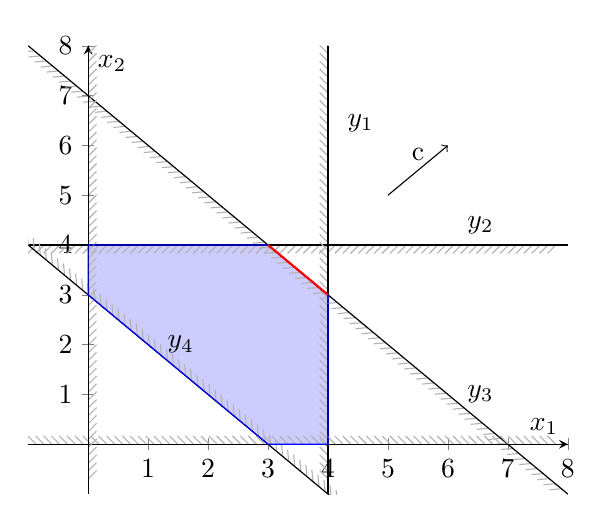
\begin{tikzpicture}
		\begin{axis}[
			axis x line=center,
			axis y line=center,
			xlabel=$x_1$,
			ylabel=$x_2$,
			xmin=-1,
			ymin=-1,
			xmax=8,
			ymax=8,
			xtick={0,1,2,...,8},
			ytick={0,1,2,...,8}
			]
			
			
			\addplot[fill=blue!20,draw=none]coordinates{(0,4)(0,3)(3,0)(4,0)(4,3)(3,4)(0,4)};
			
			
			\addPlotLDown{4} % y_1
			\node[label={20:$y_1$}] at (4,6) {};
			\addPlotLDownCoords{(4,8)(4,-1)} %y_2
			\node[label={10:$y_2$}] at (6,4) {};
			\addPlotLDown{-x + 7}; % y_3
			\node[label={0:$y_3$}] at (6,1) {};
			\addPlotRUp{-x+3}; % y_4
			\node[label={0:$y_4$}] at (1,2) {};
			
			\addPlotRUp{0}; % x_1 >= 0
			\addPlotRUpCoords{(0,8)(0,-1)}; % x_2 >= 0
			
			\addplot[fill=none,draw=blue]coordinates{(0,4)(0,3)(3,0)(4,0)(4,3)(3,4)(0,4)};
			
			\draw[black, ->] (5,5)--(6,6);
			\coordinate[label=c] (c) at (5.5,5.5);
		
			\draw[red, thick] (4,3)--(3,4);
			
		\end{axis}
	\end{tikzpicture}
\end{center}

\subsection{In the drawing from \ref{sec:1e}, you might have observed that there exist infinitely many optimal solutions. Can you argue that this is indeed true by only looking at the optimal tableau obtained in part \ref{sec:1d}?}

Yes, by performing a pivot to bring $y_1$ into basis and $y_2$ out of basis the tableau remains optimal and feasible.

\begin{minipage}{.5\textwidth}
	\centering
	\begin{tabular}{L|RR||R}
		&  y_3 & y_1 & (1)  \\
		\hline
		z   & 1 & 0 & 7 \\
		\hline
		y_4 & 1 & 0 & 4 \\
		y_2 &-1 & \fbox{$1$} & 1 \\
		x_2 & 1 &-1 & 3 \\
		x_1 & 0 & 1 & 4 \\
	\end{tabular}

(Copied from \ref{sec:1d})
\end{minipage}
$\Rightarrow$
\begin{minipage}{.5\textwidth}
	\centering
	\begin{tabular}{L|RR||R}
		&  y_3 & y_2 & (1)  \\
		\hline
		z   & 1 & 0 & 7 \\
		\hline
		y_4 & 1 & 0 & 4 \\
		y_1 &-1 & 1 & 1 \\
		x_2 & 0 & 1 & 4 \\
		x_1 & 1 &-1 & 3 \\
	\end{tabular}
\end{minipage}

\section{Problem 2:Certifying infeasibility from phase I of the Simplex Method }

\end{document}

